\documentclass[twocolumn]{article}
\usepackage{amsmath}
\usepackage{algorithm}
\usepackage{algpseudocode}
\usepackage{amsthm}
\usepackage{graphicx}
\usepackage{appendix}
\usepackage{balance}

\textwidth 6.75in
\oddsidemargin -0.10in
\textheight 9.5in
\topmargin -0.75in
\parskip 4pt

\usepackage[utf8]{inputenc} % allow utf-8 input
\usepackage[T1]{fontenc}    % use 8-bit T1 fonts
\usepackage{hyperref}       % hyperlinks
\hypersetup{
    colorlinks=true,
    linkcolor=blue,
    citecolor=blue,
    filecolor=magenta,
    urlcolor=blue,
}
\urlstyle{same}
\usepackage{url}            % simple URL typesetting
\usepackage{booktabs}       % professional-quality s
\usepackage{amsfonts}       % blackboard math symbols
\usepackage{nicefrac}       % compact symbols for 1/2, etc.
\usepackage{microtype}      % microtypography

\usepackage{tabularx}
\usepackage{booktabs}
\usepackage[]{natbib}
\usepackage{enumitem}
\usepackage{graphicx}
\usepackage{array}
\usepackage{ulem}
\usepackage{amssymb}
\usepackage{amsmath}
\usepackage{fancyhdr}
\usepackage{float}  %float allows [H] to force a Exhibit or  where you want it
% \usepackage{sans}
\usepackage{listings}
\usepackage{soul}

% Rename s and figures to exhibit
\usepackage{newfloat}
\DeclareFloatingEnvironment[%
   fileext=loe,
   name=Exhibit
]{exhibit}

\DeclareMathOperator*{\argmax}{\arg\!\max}

\AtBeginEnvironment{thebibliography}{\sloppy\hbadness=10000}
\setlength{\emergencystretch}{2em}
\raggedbottom

\begin{document}

% \title{Multivariate Financial Forecasting using the \\Chronos Time Series Foundation Models\thanks{Das is a professor of Finance and Data Science, and Goyal and Yadav are graduate students in the Leavey School of Business at Santa Clara University.}}
% \author{Sanjiv R. Das, Tarang Goyal, Mohini Yadav \\ Santa Clara University\\ \texttt{srdas@scu.edu; tgoyal@scu.edu; myadav@scu.edu}}

\title{Can Time-Series Foundation Models \\Generate Improved Multivariate Forecasts?}

\maketitle


\begin{abstract}
How capable are time series foundation models? Using Chronos-2, an open-source time-series foundation model, we evaluate pretrained time-series models for economic and financial forecasting with an emphasis on whether multivariate (MV) inputs improve accuracy relative to univariate (UV) baselines. Just as LLMs generate sequences of words, Chronos-2 is trained on thousands of time series, and generates forward sequences of data based on multivariate histories. The study covers two panels---the Magnificent-7 equities and U.S. Treasury interest rates---as well as a combined panel, using rolling monthly evaluations from 2000--2025. We vary input window lengths and forecast horizons and report RMSE and MAPE. Across datasets, MV forecasts consistently outperform UV forecasts, with especially strong gains for interest rates and meaningful improvements for equities. Series-level comparisons show MV improvements in every case, and error dispersion is generally lower under MV inputs. We also provide parameter-heatmap and time-series visualizations. However, mixing time series across equity and interest rate markets reduces forecast accuracy, indicating that adding noisy context degrades model performance. Overall, the results indicate that foundation models can leverage cross-series information to improve forecast accuracy in finance, and that the benefits are strongest when related series are modeled jointly under disciplined rolling protocols. 
% Other than using an open-source foundation model, this paper also  showcases how AI may be used for financial research. 
\end{abstract}


\section{Introduction}

Time-series forecasting in finance remains a contested area for machine learning. While deep learning has transformed NLP and computer vision, its advantage in financial forecasting is less clear. Recent studies of U.S. Treasury yield curve forecasting report that classical econometric baselines often outperform modern machine-learning models across long spans of daily data, with few learning approaches delivering competitive gains. These findings underscore an open question: when do multivariate methods provide reliable improvements over univariate forecasting? Expanding data from univariate to multivariate prompts the standard concern of whether it introduces signal or noise.

The emergence of foundation models—large, self-supervised models adapted to downstream tasks—has begun to reshape forecasting. These models promise both scale and transfer, exploiting shared structure across diverse series to improve accuracy in noisy or data-limited domains. Yet evidence from competitions and applied finance \citep{singh_yield_2025} suggests that pure deep-learning solutions often struggle without hybridization or careful engineering.

This paper evaluates if foundation-model forecasting delivers practical improvements in finance, focusing on Chronos-2, an open-source model (GitHub: \url{https://github.com/amazon-science/chronos-forecasting}). Just as large language models generate a sequence of words, Chronos-2 Chronos-2 is trained on thousands of time series, and generates forward sequences of data based on multivariate histories. We hypothesize that properly chosen multivariate (MV) inputs can help models extract cross-series information and outperform univariate (UV) baselines. We test this across two panels—the Magnificent-7 equities and U.S. Treasury rates—and a combined panel to assess if joint modeling improves results.

The contribution of the paper is threefold. First, we provide a systematic comparison of MV versus UV forecasting across equities and rates with a consistent rolling evaluation protocol. We find that the MV approach beats the UV one. Second, we examine whether MV gains differ by asset class and whether joint stock and interest rates modeling improves accuracy. In this case, we find that adding a different class of time series does not improve forecasting, highlighting that expanding the basis set for modeling does not always improve forecast accuracy. Indeed, there is a signal to noise tradeoff that applies here. additional context is not always useful. Third, we offer large-scale outputs---error metrics, forecasts with uncertainty quantiles, and visualization-ready artifacts---to support robust evaluation and downstream use. Collectively, these results clarify when foundation models add value to financial forecasting.

\subsection{Literature Review}

The literature on financial time-series forecasting spans classical econometrics, machine learning (ML), and deep learning. Standard statistical tools remain central and are documented in foundational texts \citep{shumway_time_2025}. In fixed-income, yield curve forecasting has been explored via no-arbitrage models \citep{moench_forecasting_2006} and forecast combinations \citep{caldeira_predicting_2013}. ML methods show mixed results, with recent studies indicating that classical econometric baselines often outperform ML and deep-learning models across daily data \citep{singh_yield_2025, sambasivan_statistical_2017}. Research on bond risk premia further highlights the potential and limitations of ML for term-structure prediction \citep{bianchi_bond_2020, hoogteijling_forecasting_2021}.

For equities, surveys emphasize deep learning's broad adoption but inconsistent performance across tasks \citep{sezer_financial_2019}. Comparisons between ARIMA, LSTM, and Prophet show that model choice is highly data-dependent, with traditional methods remaining competitive \citep{sunki_time_2024}. Experts argue for rigorous validation and robust benchmarks to avoid overfitting and spurious gains \citep{lopez_de_prado_advances_2018}. These themes motivate the careful use of UV baselines and out-of-sample evaluation in this study.

Recent deep-learning advances include specialized architectures like NHITS \citep{challu_nhits_2023} and time-series foundation models. Chronos is a large, self-supervised model designed for cross-domain transfer \citep{ansari_chronos_2024}. This paper tests whether MV inputs systematically improve accuracy for equities and rates using consistent rolling protocols and multiple metrics. We specifically focus on the newest generation model, Chronos-2 \citep{ansari_chronos-2_2025}.



\section{Methodology}

This section outlines our research questions and the Chronos-2 forecasting pipeline, including data scope, rolling evaluation, and analysis artifacts.

\subsection{Research Questions}

We address three questions. First, does multivariate (MV) forecasting outperform univariate (UV) methods within the Chronos-2 framework? Second, do MV gains vary between asset classes (stocks vs. interest rates)? Third, does joint modeling of stocks and rates improve accuracy over separate modeling?

\subsection{Overview of the Chronos-2 model}

Chronos-2 advances time-series foundation models by enabling zero-shot, multivariate, and covariate-informed forecasting. It moves beyond single-series histories to joint inference across related series without task-specific retraining, simplifying deployment and improving transfer to new domains. Architecturally, Chronos-2 uses a group-attention mechanism for in-context learning across series sets. A ``group'' can include multivariate variates, related targets, or targets with covariates. This design facilitates information sharing and cross-series structure learning at inference time. To build these capabilities, the model is pretrained on synthetic multivariate constructions. Chronos-2 achieves state-of-the-art results on benchmarks like GIFT-Eval and Chronos Benchmark II, particularly for covariate-conditioned tasks. The methodology transforms forecasting into a universal task via a transformer architecture and innovative pre-training (see Figure 1 in the Chronos-2 technical report, \citep{ansari_chronos-2_2025}). Key components include:
\begin{enumerate}
\item Tokenization and Robust Scaling. Data is normalized via robust scaling and a $sinh^{-1}$ transformation to stabilize variance. Categorical covariates are encoded, and data is augmented with meta-features like a relative time index and a binary mask for missing values.
\item Patch-Based Representation. Chronos-2 divides the series and meta-features into non-overlapping patches of length $P$. These are mapped into embeddings via a residual network, with a REG token serving as an attention sink between history and future patches.
\item Core Architecture: Time and Group Attention. The encoder-only transformer alternates between: (a) Time Attention, which aggregates temporal information using RoPE, and (b) Group Attention, the core innovation allowing cross-series information sharing within a group at each patch index.
\item Multivariate and Covariate Integration. Tasks are managed via Group IDs. In multivariate tasks, related variates share an ID to model dependencies. Known future covariates are included in the future input matrix $W$, allowing for conditioned forecasts.
\item Training and Quantile Forecasting. Trained in two stages (context lengths up to 8192), the model uses quantile regression to produce probabilistic forecasts across 21 quantiles. Its in-context learning capabilities are largely derived from synthetic multivariate datasets.
\end{enumerate}

In sum, the methodology of Chronos-2 involves an encoder-only transformer architecture that utilizes a novel group attention mechanism and robust scaling to perform zero-shot univariate, multivariate, and covariate-informed forecasting by sharing information across related time series in-context.

\subsection{Implementation}

The data consist of three panels: the Magnificent-7 stocks (AAPL, AMZN, GOOGL, MSFT, NFLX, NVDA, TSLA) ($K=7$), Treasury interest rates for ten different maturities ($K=10$), and a combined panel of all series ($K=17$). This design supports both within-group and cross-group forecasting comparisons.

We use input window lengths $n \in \{126, 252, 504, 756\}$ trading days, and forecast horizons $m \in \{21, 63\}$ trading days to cover short to medium histories (0.5 to 3 years) and near- to mid-term prediction horizons (1 to 3 months).

The evaluation period spans 2000--2025 with monthly rolling forecasts to reflect realistic re-estimation and deployment cadence. Forecast accuracy is measured using RMSE (root mean squared error) and MAPE (mean absolute percentage error) to capture both scale-dependent and scale-free error behavior. 

To assess temporal robustness, we compare performance across pre-2023 and post-2023 regimes using a training cutoff that separates the sample. We will also argue that this is a check on information leakage in the model. 

\section{Results}

\subsection{Forecasts within asset classes}

This paper examines improvements when using multivariate (MV) instead of univariate (UV) forecasting. Table~\ref{tab:avg-performance} summarizes performance by dataset and mode across all tickers and period combinations. MV forecasts outperform UV for both rates and stocks, showing significant MAPE and RMSE reductions in rates and moderate reductions in stocks. Forecast error standard deviation is also lower for MV. Overall, multivariate models in Chronos-2 provide robust, easily implemented forecasts.

\begin{table}[H]
\centering
\caption{\label{tab:avg-performance} \small Average performance by dataset and mode. Lower mean error across all experiments (for values of input length $n=\{126, 252, 504, 756\}$, and forecast period $m=\{21, 63\}$) measured by MAPE and RMSE is better. Data for the rolling periods is from 2000 through 2025. Predictions periods begin 3 years after the start of the dataset. }
\resizebox{\columnwidth}{!}{%
\begin{tabular}{llrrrr}
\toprule
Dataset & Mode & \multicolumn{2}{c}{MAPE} & \multicolumn{2}{c}{RMSE} \\
& & mean & std & mean & std \\
\midrule
Rates  & MV & 0.0497 & 0.1673 & 0.0418 & 0.0445 \\
Rates  & UV & 0.1233 & 0.2213 & 0.1865 & 0.1783 \\
Stocks & MV & 0.0706 & 0.0728 & 3.9619 & 9.0440 \\
Stocks & UV & 0.0844 & 0.0834 & 5.0395 & 11.5710 \\
\bottomrule
\end{tabular}
}
\end{table}

Table~\ref{tab:uv-mv-comparison} reports UV vs.\ MV results by series. MV improves MAPE and RMSE for every rate and stock. This clear win suggests that additional related time series add value when used within a pre-trained foundation time series model.

\begin{table*}[t]
\centering
\caption{\label{tab:uv-mv-comparison} \small UV vs.\ MV comparison by series (lower is better). Improvements are mean UV error minus mean MV error. Results are averaged across values of input length $n=\{126, 252, 504, 756\}$, and forecast period $m=\{21, 63\}$. Data for the rolling periods is from 2000 through 2025. Predictions periods begin 3 years after the start of the dataset. 
}
\resizebox{\textwidth}{!}{%
\begin{tabular}{llrrrrrr}
\toprule
Dataset & Series & MAPE\,(MV) & MAPE\,(UV) & RMSE\,(MV) & RMSE\,(UV) & MAPE\,Imp. & RMSE\,Imp. \\
\midrule
Rates & DGS3MO & 0.2355 & 0.3186 & 0.0618 & 0.1227 & 0.0831 & 0.0609 \\
Rates & DGS6MO & 0.0833 & 0.1770 & 0.0455 & 0.1257 & 0.0937 & 0.0802 \\
Rates & DGS1   & 0.0572 & 0.1326 & 0.0454 & 0.1424 & 0.0754 & 0.0970 \\
Rates & DGS2   & 0.0334 & 0.1270 & 0.0413 & 0.1845 & 0.0936 & 0.1432 \\
Rates & DGS3   & 0.0243 & 0.1181 & 0.0388 & 0.2068 & 0.0938 & 0.1680 \\
Rates & DGS5   & 0.0171 & 0.0972 & 0.0359 & 0.2232 & 0.0801 & 0.1873 \\
Rates & DGS7   & 0.0134 & 0.0827 & 0.0345 & 0.2278 & 0.0693 & 0.1933 \\
Rates & DGS10  & 0.0114 & 0.0703 & 0.0344 & 0.2184 & 0.0589 & 0.1840 \\
Rates & DGS20  & 0.0099 & 0.0572 & 0.0364 & 0.2120 & 0.0473 & 0.1756 \\
Rates & DGS30  & 0.0113 & 0.0520 & 0.0442 & 0.2012 & 0.0407 & 0.1570 \\
\midrule
Stocks & AAPL  & 0.0599 & 0.0720 & 3.3016  & 4.1563  & 0.0121 & 0.8547 \\
Stocks & AMZN  & 0.0567 & 0.0707 & 3.0825  & 4.0517  & 0.0140 & 0.9692 \\
Stocks & GOOGL & 0.0478 & 0.0635 & 3.1803  & 4.0070  & 0.0157 & 0.8267 \\
Stocks & MSFT  & 0.0368 & 0.0466 & 4.2003  & 6.1519  & 0.0098 & 1.9516 \\
Stocks & NFLX  & 0.1040 & 0.1145 & 1.7871  & 2.0192  & 0.0105 & 0.2321 \\
Stocks & NVDA  & 0.0906 & 0.1107 & 1.5994  & 1.8420  & 0.0201 & 0.2426 \\
Stocks & TSLA  & 0.1098 & 0.1242 & 13.6796 & 16.7870 & 0.0144 & 3.1074 \\
\bottomrule
\end{tabular}
}
\end{table*}

Figure~\ref{fig:parameter_heatmap} breaks down errors by input length $n$ and forecast length $m$. MV consistently yields smaller errors than UV. Accuracy predictably decreases for the 63-day horizon compared to 21 days, but input length $n$ (from six months to three years) has little impact on results.

\begin{figure*}[t]
\centering
{\bf Rates forecast MAPE}\\
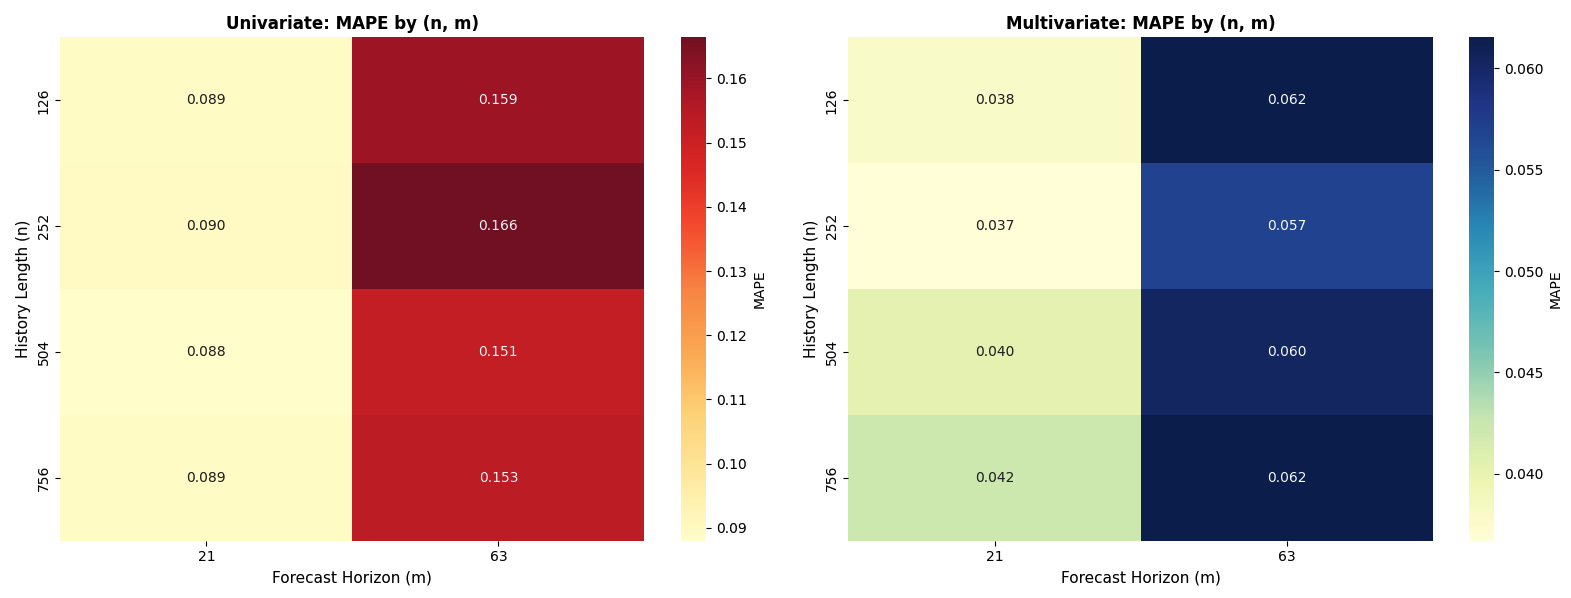
\includegraphics[width=\textwidth]{rates_mape.png}
{\bf Stocks forecast MAPE}\\
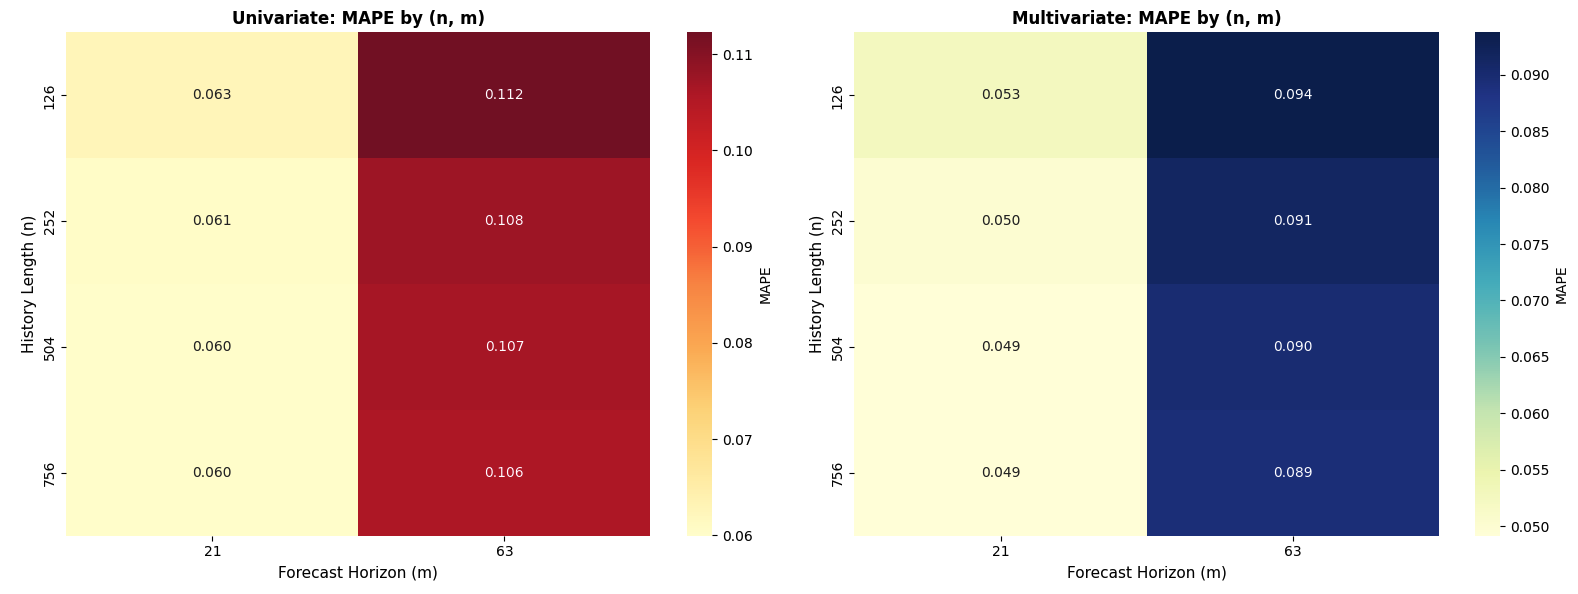
\includegraphics[width=\textwidth]{stocks_mape.png}
\caption{\label{fig:parameter_heatmap} \small Parameter heatmap comparing MV and UV forecasting accuracy across window lengths and horizons (based on MAPE). The upper plot is for Rates and the lower one is for Stocks. In each plot, the left side is for the 21 working day forecast (1 month forecast) and the right side is for the 63 working day forecast (3 month forecast)}
\end{figure*}

MAPE error time series are shown in Figure~\ref{fig:uv_mv_time_series}. UV errors are consistently higher, especially for interest rates. Errors appear to rise at higher asset levels despite using percentage metrics. Overall, Figures~\ref{fig:parameter_heatmap} and \ref{fig:uv_mv_time_series} confirm that MV forecasts are more accurate.

\begin{figure*}[t]
\centering
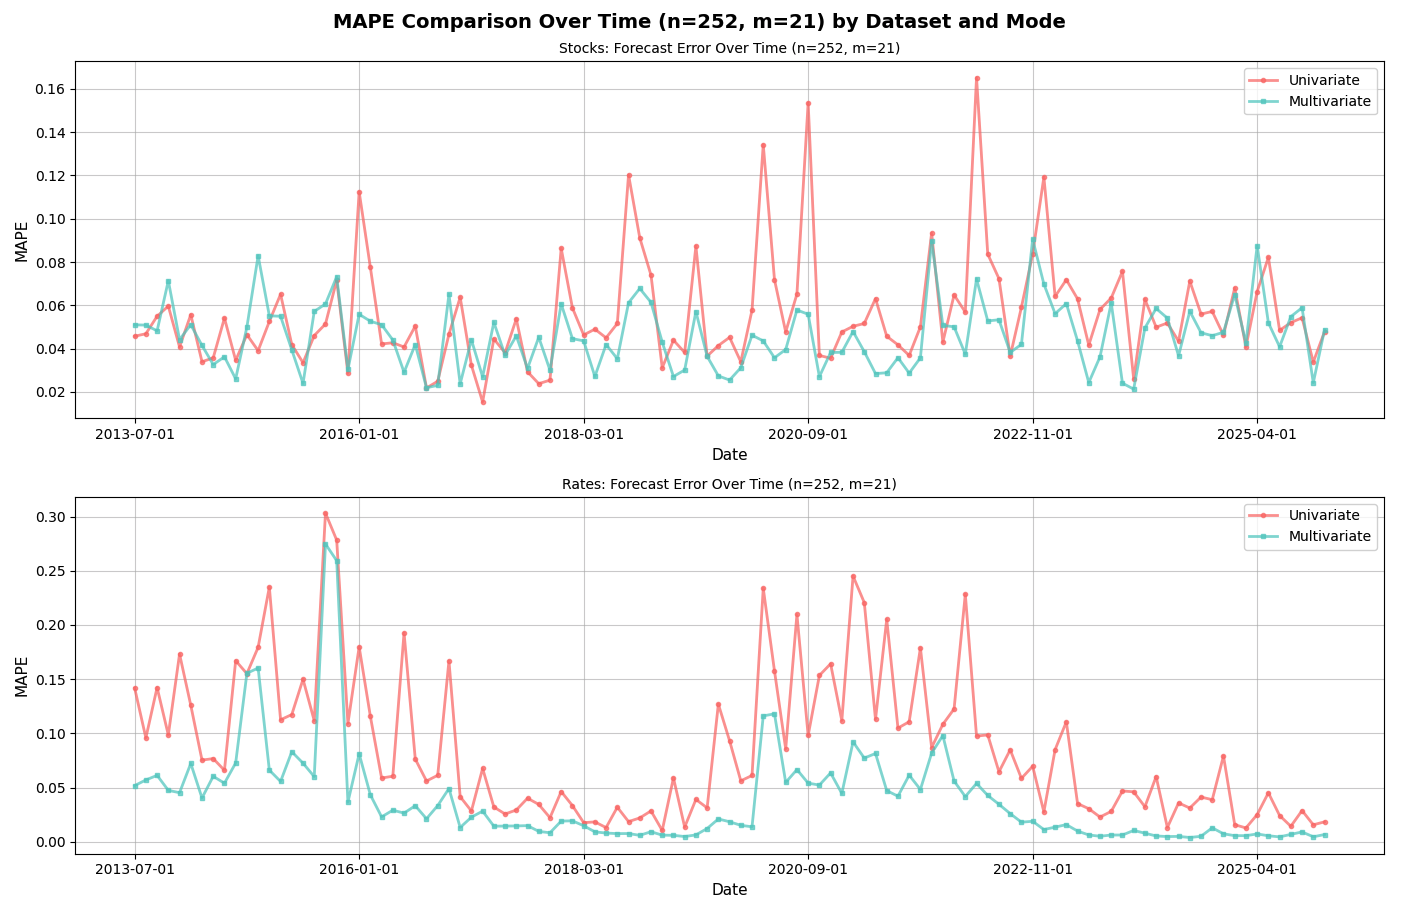
\includegraphics[width=\textwidth]{error_series.png}
\caption{\label{fig:uv_mv_time_series} \small Time series of MV and UV MAPE errors over the evaluation period. This is for the dataset running from July 2010 through December 2025. }
\end{figure*}

\subsection{Forecasts with combined asset classes}

This section assesses a "small world" model combining rates and stocks to see if cross-domain data improves results. We test whether forecasting a series using both families of data exploits additional cross-market information.

Using the period July 2010 to December 2025 for consistency, Table \ref{tab:uv-mv-combined} shows that cross-market data does not improve forecasts and may slightly degrade quality by adding noise. In foundation models, this unrelated context may distract the model from the target domain.

\begin{table*}
\centering
\caption{\label{tab:uv-mv-combined} \small Combined dataset forecasts. UV vs.\ MV comparison by series (lower is better). Improvements are mean UV error minus mean MV error. Results are averaged across values of input length $n=\{126, 252, 504, 756\}$, and forecast period $m=\{21, 63\}$. Data is for the period July 2010 through December 2025, the period when there is complete data for all stocks and rates. For comparison, we show the results when forecasts are based on the individual datasets for Rates and Stocks, as well as when forecasts are based on the combination of both datasets. Predictions periods begin 3 years after the start of the dataset. (As expected the UV forecast errors do not change.) 
}
\resizebox{\textwidth}{!}{%
\begin{tabular}{llrrrrrr}
\toprule
Dataset & Series & MAPE\,(MV) & MAPE\,(UV) & RMSE\,(MV) & RMSE\,(UV) & MAPE\,Imp. & RMSE\,Imp. \\
\midrule
Rates & DGS3MO & 0.2304 & 0.2849 & 0.0597 & 0.1052 & 0.0545 & 0.0455 \\
Rates & DGS6MO & 0.0937 & 0.1714 & 0.0500 & 0.1179 & 0.0777 & 0.0679 \\
Rates & DGS1 & 0.0609 & 0.1289 & 0.0475 & 0.1363 & 0.0680 & 0.0888 \\
Rates & DGS2 & 0.0366 & 0.1216 & 0.0426 & 0.1727 & 0.0850 & 0.1301 \\
Rates & DGS3 & 0.0257 & 0.1111 & 0.0378 & 0.1883 & 0.0854 & 0.1505 \\
Rates & DGS5 & 0.0185 & 0.0959 & 0.0341 & 0.2025 & 0.0774 & 0.1684 \\
Rates & DGS7 & 0.0144 & 0.0843 & 0.0321 & 0.2086 & 0.0699 & 0.1765 \\
Rates & DGS10 & 0.0128 & 0.0759 & 0.0325 & 0.2045 & 0.0631 & 0.1720 \\
Rates & DGS20 & 0.0116 & 0.0628 & 0.0353 & 0.1993 & 0.0512 & 0.1640 \\
Rates & DGS30 & 0.0122 & 0.0573 & 0.0396 & 0.1923 & 0.0451 & 0.1527 \\
\midrule
Stocks & AAPL  & 0.0500 & 0.0621 & 5.6015  & 7.1124  & 0.0121 & 1.5109 \\
Stocks & AMZN  & 0.0462 & 0.0617 & 5.2798  & 7.0294  & 0.0155 & 1.7496 \\
Stocks & GOOGL & 0.0411 & 0.0545 & 4.8211  & 6.0685  & 0.0134 & 1.2474 \\
Stocks & MSFT  & 0.0305 & 0.0453 & 6.6967  & 10.1334 & 0.0148 & 3.4367 \\
Stocks & NFLX  & 0.0792 & 0.0902 & 3.0946  & 3.4715  & 0.0110 & 0.3769 \\
Stocks & NVDA  & 0.0743 & 0.0980 & 2.7598  & 3.3253  & 0.0237 & 0.5655 \\
Stocks & TSLA  & 0.1090 & 0.1258 & 16.6789 & 20.7258 & 0.0168 & 4.0469 \\
\bottomrule
Dataset & Series & MAPE\,(MV) & MAPE\,(UV) & RMSE\,(MV) & RMSE\,(UV) & MAPE\,Imp. & RMSE\,Imp. \\
\midrule
Combined & DGS3MO & 0.2392 & 0.2849  & 0.0655  & 0.1052  & 0.0457  & 0.0397  \\
Combined & DGS6MO & 0.1002 & 0.1714  & 0.0543  & 0.1179  & 0.0712  & 0.0636  \\
Combined & DGS1    & 0.0671 & 0.1289  & 0.0518  & 0.1363  & 0.0618  & 0.0845  \\
Combined & DGS2    & 0.0392 & 0.1216  & 0.0440  & 0.1727  & 0.0824  & 0.1287  \\
Combined & DGS3    & 0.0256 & 0.1111  & 0.0374  & 0.1883  & 0.0855  & 0.1509  \\
Combined & DGS5    & 0.0189 & 0.0959  & 0.0346  & 0.2025  & 0.0770  & 0.1679  \\
Combined & DGS7    & 0.0145 & 0.0843  & 0.0329  & 0.2086  & 0.0698  & 0.1757  \\
Combined & DGS10  & 0.0126 & 0.0759  & 0.0327  & 0.2045  & 0.0633  & 0.1718  \\
Combined & DGS20  & 0.0121 & 0.0628  & 0.0367  & 0.1993  & 0.0507  & 0.1626  \\
Combined & DGS30  & 0.0129 & 0.0573  & 0.0414  & 0.1923  & 0.0444  & 0.1509  \\
\midrule
Combined & AAPL    & 0.0519 & 0.0621  & 5.6524  & 7.1124  & 0.0102  & 1.4600  \\
Combined & AMZN    & 0.0470 & 0.0617  & 5.1538  & 7.0294  & 0.0147  & 1.8756  \\
Combined & GOOGL   & 0.0399 & 0.0545  & 4.5781  & 6.0685  & 0.0146  & 1.4904  \\
Combined & MSFT    & 0.0318 & 0.0453  & 6.7621  & 10.1334 & 0.0135  & 3.3713  \\
Combined & NFLX    & 0.0786 & 0.0902  & 3.0877  & 3.4715  & 0.0116  & 0.3838  \\
Combined & NVDA    & 0.0761 & 0.0980  & 2.8012  & 3.3253  & 0.0219  & 0.5241  \\
Combined & TSLA    & 0.1114 & 0.1258  & 16.8843 & 20.7258 & 0.0144  & 3.8415 \\
\bottomrule
\end{tabular}
}
\end{table*}

\subsection{Leakage}

We address potential "leakage"—the risk that test data appeared in pre-training. Chronos models exclude the financial series used here. Chronos-2 \citep{ansari_chronos-2_2025} focuses on training diversity, using synthetic data via TSI \citep{bahrpeyma_methodology_2021} and TCM \citep{runge_causal_2023} approaches. While the original model \citep{ansari_chronos_2024} utilized some macroeconomic \citep{godahewa_monash_2021} and financial datasets \citep{makridakis_m4_2020}, they did not include our specific series, especially post-2023 data.

Two points counter leakage: (i) if leakage existed, MV and UV forecasts would show little difference, yet significant gains appear in Tables \ref{tab:avg-performance} through \ref{tab:uv-mv-combined}; (ii) post-2023 forecasts—which could not be in training—are actually more accurate (Figure \ref{fig:pre_post_2023}), especially for rates. These results suggest leakage is not a factor and that foundation models excel when using multivariate series within the same contextual domain.

\begin{figure*}
\centering
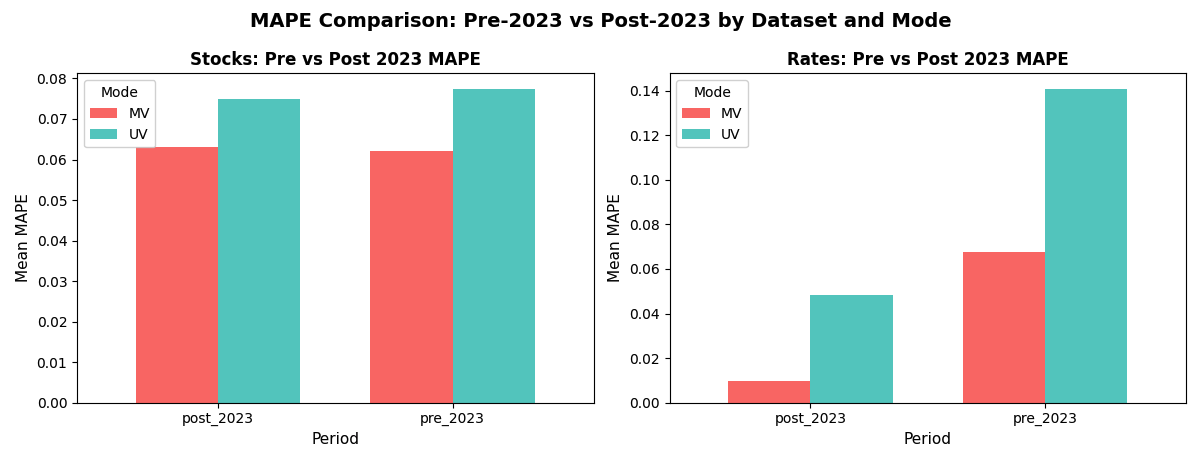
\includegraphics[width=\textwidth]{pre_post_2023_cutoff.png}
\caption{\small Comparison of forecast accuracy pre-2023 and post-2023. Data used is for the period July 2010 through December 2025. }
\label{fig:pre_post_2023}
\end{figure*}


\section{Concluding Discussion}

This paper evaluates Chronos-2 as a foundation-model for financial forecasting, specifically testing if multivariate (MV) inputs improve accuracy over univariate (UV) baselines. Across equities and U.S. Treasury rates, MV forecasts consistently outperform UV counterparts, showing significant MAPE and RMSE reductions. These results demonstrate that foundation models effectively capitalize on cross-series information when inputs are properly structured. These results are some of the first that support this class of foundation models for use in financial forecasting. 

Our findings contribute to the debate on machine learning in finance. Consistent with evidence that classical benchmarks are resilient, our results show that gains depend on leveraging multivariate structures within disciplined rolling protocols. The primary advantage of foundation models likely stems from their ability to transfer information across related series and accommodate numerous inputs—a task often difficult for traditional econometric models.

Several limitations remain. This study focuses on one foundation model and a specific asset set. The evaluation uses fixed windows and horizons; different data frequencies or rolling cadences might yield alternative results. Furthermore, while we report standard error metrics, specific use cases may require deeper analysis of tail risk, directional accuracy, and economic utility.

Future research can extend this framework in three directions. First, expanding to a larger "world" panel—including macroeconomics, commodities, and international data—could test transfer learning at scale. Second, integrating uncertainty calibration, such as conformal prediction, would enhance forecast interval reliability. Finally, hybrid designs merging econometric baselines with foundation-model embeddings may provide robust performance alongside interpretability.


\clearpage

\balance
\bibliographystyle{chicago}
\bibliography{ts}

\clearpage
\appendix

\section{Appendix: AI-Driven Workflow to Generate the Paper}
\label{ai_workflow}

This appendix outlines how the paper was produced with the assistance of Artificial Intelligence.

% The project began informally in January 2026 when Professor Das outlined the work to the students. The students delivered the completed code in a single Google Colab notebook by late February. For the purpose of this workflow, the ``formal'' writing process began at that point. The students utilized Gemini to assist in code development. Subsequently, the professor modified the code to utilize GPU resources and rerun the analyses. OpenAI Prism was then used to draft the paper over several hours of interaction, followed by final human editing. Work was completed in 2 months.

\section*{Detailed Workflow Step-by-Step}

Each step below was followed by human review, if AI was involved. 

\begin{enumerate}[label=\arabic*.]
    \item \textbf{Conceptualization:} Students are provided an initial outline.
    \item \textbf{Initial Coding:} Students prepare a Google Colab notebook with assistance from Gemini.
    \item \textbf{Refinement:} The professor updates the notebook, modularizing the code and updating logic, also utilizing Gemini for coding assistance.
    \item \textbf{Data Preparation:} Results are finalized in Colab, consisting of printed dataframes, plots, and textual outputs.
    \item \textbf{Environment Setup:} A \LaTeX{} shell for the paper is established in OpenAI Prism (\url{https://openai.com/prism/}).
    \item \textbf{Outlining:} The structure is set up with blank sections: Introduction, Methodology, Results, and Concluding Discussion (including relevant subsections).
    \item \textbf{Table Conversion:} Printed dataframes from Colab are fed into Gemini with prompts to convert them into \LaTeX{} tables. These are then integrated into the Results section.
    \item \textbf{Visuals:} Figures are added to the project folder, and the corresponding \LaTeX{} code for figure inclusion is written.
    \item \textbf{Drafting Results:} Prism is tasked with drafting text for the Results section to explain the tables and figures. Notably, the underlying model (GPT-5.2) inferred results directly from the tables to generate the write-up.
    \item \textbf{Methodology:} The Chronos-1 and Chronos-2 papers, along with experiment descriptions from the Colab notebook, are uploaded to Gemini. Gemini generates the Methodology section, which is then moved to the draft.
    \item \textbf{Specific Subsections:} A subsection on data leakage is added; the reasoning is provided by the authors while the LLM handles the prose.
    \item \textbf{Literature Review (Part 1):} A Bib\TeX{} file from Zotero is uploaded. Prism is prompted to generate a literature review based on the citations as they relate to the Methodology and Results.
    \item \textbf{Introduction and Literature Review (Part 2):} Previously published related papers are uploaded. Prism generates the Introduction and updates the literature review for context.
    \item \textbf{Conclusions:} Using the full paper as context, Prism generates the Concluding Discussion.
    \item \textbf{Abstract:} Prism is prompted to synthesize an abstract for the completed draft.
    \item \textbf{Human Editing:} Final human-led editing passes are performed to improve narrative flow, reformat the \LaTeX{} layout, and ensure technical accuracy.
\end{enumerate}

\subsection*{Self Review and Revision Process}
Gemini was also utilized to generate a mock referee report (\texttt{review.pdf}). This report informed a response document (\texttt{responses.md}) created with the following prompt: 
\begin{quote}
    \textit{``Please read the file ‘review.pdf‘ which is a referee report on the paper ‘chronos2.pdf‘ – then suggest changes and improvements to the paper in a document titled ‘response.md‘ that outlines the changes in response to cited sections of ‘review.pdf‘ as a response note to the review.''}
\end{quote}
Final edits were made to the manuscript based on these AI-suggested improvements. 

% The code and files for the paper have been made public on GitHub: \url{https://github.com/srdas/timeseries-fm/tree/main}.


\end{document}
